\chapter{Methodology}
\label{ch:method}

This chapter describes each stage of the pipeline: its purpose, the algorithm it runs and the mathematics behind it, illustrated with examples from real runs of the system. The statistical theory of the conformal layer is developed separately in Chapter~\ref{ch:stats}.

% --------------------------------------------------------------------------
\section{Claim Decomposition}
\label{sec:decomp}

A single sentence often bundles several facts, some true and some false: \emph{``Tim Cook replaced Steve Jobs in 2011 and founded Apple''} is half right. Verifying the sentence as a whole would force one verdict onto two facts. Decomposition splits the input into \emph{atomic claims}, each with exactly one checkable proposition.

\paragraph{Algorithm.}
\begin{enumerate}[itemsep=0.2em]
  \item \textbf{Atomic fast path.} If $T$ is a single sentence of at most 15 words and contains none of a conservative list of clause markers (\code{;}, \code{,}, \emph{and}, \emph{but}, \emph{which}, \emph{because}, \emph{who}, \emph{that}, \emph{with}, \dots), it is already atomic and is returned unchanged, with no LLM call.
  \item \textbf{LLM decomposition.} Otherwise an LLM returns a JSON array of atomic facts under two mandatory rules. \emph{Coreference resolution}: every pronoun and implicit reference is replaced by the explicit proper noun, so each claim can be verified on its own. \emph{Polarity preservation}: the truth value and negations of the original text are kept verbatim, and the model must never ``correct'' a false statement into a true one, which would silently delete the hallucination the detector is meant to find.
  \item \textbf{Fallback.} If the LLM call fails or returns invalid JSON, the text is split into sentences with the NLTK tokenizer.
\end{enumerate}

\begin{table}[htbp]
\centering
\caption{Claim decomposition examples.}
\label{tab:decomp}
\small
\begin{tabularx}{\textwidth}{@{}XlX@{}}
\toprule
Input & Route & Output claims \\
\midrule
\emph{Juneau is the capital of Alaska.} & fast path & \emph{Juneau is the capital of Alaska.} \\
\emph{Albert Einstein was born in 1950 in San Francisco, and he won the Nobel Prize in Literature in 1980.} & LLM & \emph{Albert Einstein was born in 1950.}; \emph{Albert Einstein was born in San Francisco.}; \emph{Albert Einstein won the Nobel Prize in Literature in 1980.} \\
\bottomrule
\end{tabularx}
\end{table}

% --------------------------------------------------------------------------
\section{Query Generation}
\label{sec:querygen}

Searching for the whole claim string returns noisy results; searching for the \emph{entities} the claim is about retrieves the encyclopedia articles that contain the deciding fact. This stage maps a claim to at most three queries, a domain (\emph{general} or \emph{scientific}) and a flag saying whether the claim depends on the present date.

A \textbf{fast path} handles short claims without ambiguous pronouns by regular expressions over common relational patterns (\emph{is the co-founder of}, \emph{was born in}, \emph{was directed by}, \emph{is a}, \dots): the subject and the capitalised object become the queries. Claims about creative works (\emph{album}, \emph{film}, \emph{series}, \dots) and claims using epithets (\emph{``the father of''}) are excluded, because they need disambiguation. Otherwise an \textbf{LLM path} is used, instructed to disambiguate titles (e.g.\ \emph{``Pixels (2015 film)''}), to resolve implicit references and to flag claims about the present. For temporal claims the evidence text is later prefixed with the current date, so that the arbiter can reason about recency.

\begin{table}[htbp]
\centering
\caption{Query generation examples.}
\label{tab:queries}
\small
\begin{tabularx}{\textwidth}{@{}XlX@{}}
\toprule
Claim & Route & Queries \\
\midrule
\emph{Barack Obama was born in Hawaii.} & fast path & \code{["Barack Obama", "Hawaii"]} \\
\emph{Bones is a television series.} & LLM (creative work) & \code{["Bones (TV series)"]} \\
\emph{The 8th president of the United States is buried in Kinderhook, New York.} & LLM & \code{["Martin Van Buren", "Kinderhook (town) New York"]} \\
\bottomrule
\end{tabularx}
\end{table}

% --------------------------------------------------------------------------
\section{Evidence Retrieval}
\label{sec:retrieval}

Evidence is collected from complementary sources, all fetched concurrently:
\begin{itemize}[itemsep=0.2em]
  \item \textbf{Wikipedia} (per query): the top two search results, with auto-suggestion disabled (it silently replaces titles), disambiguation pages resolved to their first option, and reference sections removed.
  \item \textbf{arXiv} (scientific claims only): up to three abstracts per query.
  \item \textbf{Web search} (once per claim, on the full claim text): six search engines are queried in parallel and the first to answer is used, with at most three results, capped at 5\,s so that a blocked engine can never stall the pipeline.
\end{itemize}

\paragraph{Chunking.} Wikipedia text is split into sentences and grouped into overlapping windows of five sentences with stride three. Window $j$ covers sentences $3j+1, \dots, 3j+5$, so consecutive windows share two sentences, and any fact stated across two adjacent sentences is contained whole in some window. Each window is one candidate paragraph.

\paragraph{Claim-echo filtering.} A web search for the exact claim frequently returns pages that merely quote it, including fact-checks that quote a false claim before debunking it. An NLI model reads a verbatim quote as perfect entailment, so a false claim could ``support itself''. Let $W(x)$ be the set of lower-cased word tokens of a text $x$. A sentence $s$ of a web snippet is removed if
\begin{equation}
  \frac{\lvert W(c) \cap W(s) \rvert}{\lvert W(c) \rvert} \ge 0.8,
\end{equation}
and a snippet left with fewer than eight tokens is dropped. Encyclopedic text is never filtered, since a Wikipedia sentence that closely matches a claim is genuine support, not an echo. In the evaluation the filter removed at least one web snippet for 37 of the 600 claims.

% --------------------------------------------------------------------------
\section{Hybrid Re-Ranking}
\label{sec:rerank}

A query typically returns dozens of candidate paragraphs; only the $k = 3$ most relevant are passed to the NLI model. Two complementary relevance signals are combined.

\paragraph{Dense similarity.} Claim and paragraphs are embedded with \code{all-MiniLM-L6-v2}~\citep{reimers2019sbert}, a six-layer sentence Transformer producing 384-dimensional vectors. For token embeddings $\mathbf{h}_1, \dots, \mathbf{h}_L$ the sentence embedding is the normalised mean
\begin{equation}
  \bar{\mathbf{h}} = \frac{1}{L} \sum_{t=1}^{L} \mathbf{h}_t, \qquad \mathbf{e} = \frac{\bar{\mathbf{h}}}{\lVert \bar{\mathbf{h}} \rVert_2},
\end{equation}
and relevance is the cosine similarity, which for unit vectors is a dot product: $\operatorname{sim}(\mathbf{c}, \mathbf{e}) = \mathbf{c}^\top \mathbf{e} \in [-1, 1]$.

\paragraph{Sparse similarity (BM25).} For a claim with tokens $t_1, \dots, t_Q$ and $N$ candidate paragraphs, the Okapi BM25 score~\citep{robertson2009bm25} of paragraph $d$ is
\begin{equation}
  \operatorname{BM25}(d, c) = \sum_{j=1}^{Q} \operatorname{IDF}(t_j) \cdot \frac{f(t_j, d)\,(k_1 + 1)}{f(t_j, d) + k_1 \left( 1 - b + b\, \dfrac{\lvert d \rvert}{\text{avgdl}} \right)},
\end{equation}
\begin{equation}
  \operatorname{IDF}(t) = \ln \frac{N - n(t) + 0.5}{n(t) + 0.5},
\end{equation}
where $f(t, d)$ is the term frequency, $\lvert d \rvert$ the paragraph length, $\text{avgdl}$ the mean length, $n(t)$ the number of candidates containing $t$, $k_1 = 1.5$ and $b = 0.75$. The fraction is increasing and bounded in $f$, tending to $k_1 + 1$, so repeating a word has diminishing returns, and the factor in $\lvert d \rvert$ penalises long paragraphs. A term in more than half the candidates would receive a negative IDF; such values are replaced by a quarter of the mean IDF.

\paragraph{Reciprocal rank fusion.} Cosine similarity lies in $[-1,1]$ and BM25 is unbounded, so the two are combined through ranks. With $r_{\text{dense}}(d)$ and $r_{\text{bm25}}(d)$ the 1-based ranks,
\begin{equation}
  \operatorname{RRF}(d) = \frac{1}{\kappa + r_{\text{dense}}(d)} + \frac{1}{\kappa + r_{\text{bm25}}(d)}, \qquad \kappa = 60.
\end{equation}
Because $1/(\kappa + r)$ is convex and flat for large $\kappa$, a paragraph ranked well by \emph{both} signals beats one ranked first by only one of them. Paragraphs are then visited in decreasing RRF order and the first three that pass a relevance floor ($\operatorname{sim} \ge 0.20$ or $\operatorname{BM25} > 1.0$) are kept. If none qualifies, retrieval returns nothing rather than feeding unrelated text to the verifier.

\paragraph{Worked example.} For the FEVER claim \emph{``Bones is a cuisine''} (query \code{["Bones"]}), 68 unique candidates were retrieved. The top paragraph, a web result on \emph{``bone swimming cuisine''}, was second by dense similarity and first by BM25, so
\[
  \operatorname{RRF} = \frac{1}{60 + 2} + \frac{1}{60 + 1} = 0.016129 + 0.016393 = 0.032522.
\]
A Wikipedia paragraph on the femur, only eighth by dense similarity but second by BM25, entered the top three: fusion rewards agreement between the rankings.

% --------------------------------------------------------------------------
\section{NLI Evidence Scoring}
\label{sec:nli}

\paragraph{The model.} The verifier is \code{facebook/bart-large-mnli}: BART-large~\citep{lewis2020bart} (12 encoder and 12 decoder layers, hidden size 1{,}024, about 407M parameters) fine-tuned on MultiNLI~\citep{williams2018mnli}. The evidence is the premise and the claim the hypothesis. The final decoder state at the end-of-sequence token, $\mathbf{h}_{\text{eos}} \in \mathbb{R}^{1024}$, is mapped to three logits by a two-layer head,
\begin{equation}
  \mathbf{z} = \mathbf{W}_2 \tanh(\mathbf{W}_1 \mathbf{h}_{\text{eos}} + \mathbf{b}_1) + \mathbf{b}_2,
\end{equation}
which are normalised by softmax:
\begin{equation}
  \hat{\pi}_y = \frac{\exp(z_y)}{\sum_{y'} \exp(z_{y'})}, \qquad \hat{y} = \argmax_{y \in \Y} \hat{\pi}_y.
\end{equation}

\paragraph{Scoring snippets separately.} If all snippets are concatenated into one premise, the decisive sentence is surrounded by background text and decisive entailments collapse towards \emph{neutral} (\emph{context dilution}). Each snippet $e_i$ is therefore scored on its own, giving $\hat{\bm{\pi}}(e_i)$, and the judgements are combined in three steps. A snippet is \emph{decisive} for label $y$ when $\hat{\pi}_y(e_i) \ge \tau = 0.80$.

\paragraph{Step 1: source conflict.} With $S = \max_i \hat{\pi}_{\text{sup}}(e_i)$ and $K = \max_i \hat{\pi}_{\text{con}}(e_i)$, sources genuinely disagree when
\begin{equation}
  S \ge 0.85 \;\wedge\; K \ge 0.85 \;\wedge\; \lvert S - K \rvert < 0.12 .
\end{equation}
The verdict is then \Unk, and the arbiter is told that the sources conflict.

\paragraph{Step 2: the corroboration rule.} Support and contradiction are not equally reliable. MNLI-trained models often assign a confident contradiction to a snippet that is merely adjacent to the claim, because a premise describing a different situation was usually labelled a contradiction in training. On the 600 evaluation claims, the number of decisive contradicting snippets turned out to be the strongest available signal of whether a refutation is real (Table~\ref{tab:corroboration}, Figure~\ref{fig:corroboration}).

\begin{table}[htbp]
\centering
\caption{Reliability of NLI refutations by the number of decisive contradicting snippets (600 claims).}
\label{tab:corroboration}
\begin{tabular}{@{}lccc@{}}
\toprule
Decisive contradicting snippets & Claims & Claim actually false & Refutation wrong \\
\midrule
1 & 99 & 70 & 29\% \\
2 & 62 & 55 & 11\% \\
3 or more & 113 & 108 & 4\% \\
decisive support also present & 29 & 9 & 69\% \\
\bottomrule
\end{tabular}
\end{table}

\begin{figure}[htbp]
\centering
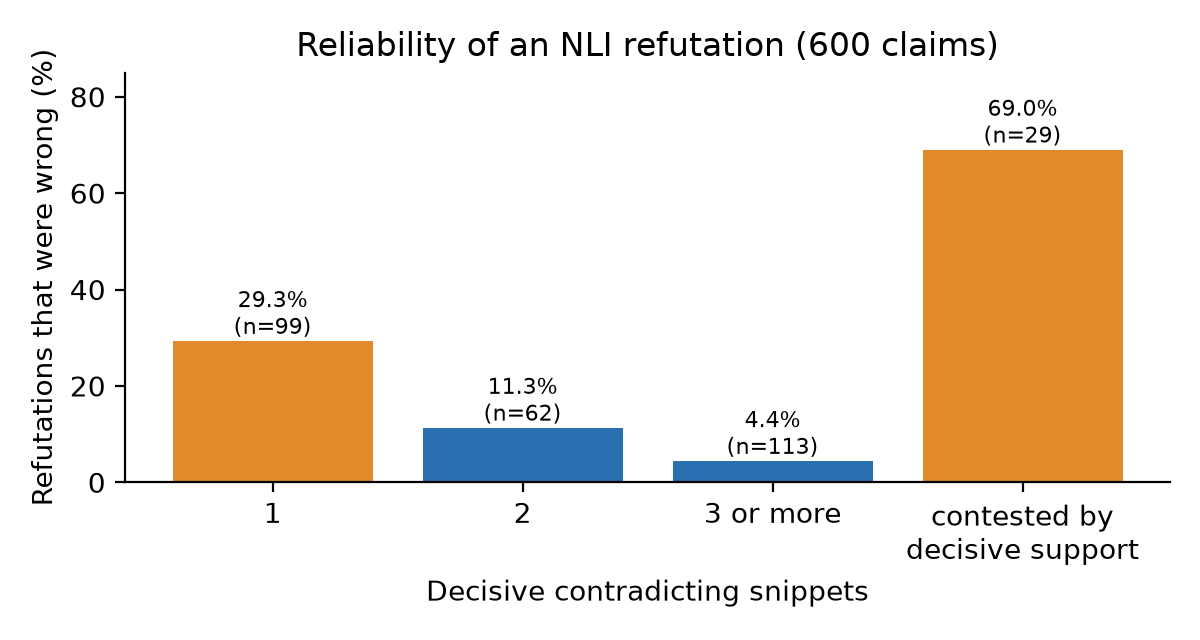
\includegraphics[width=0.72\textwidth]{corroboration.png}
\caption{Share of NLI refutations that were wrong, by the number of decisive contradicting snippets.}
\label{fig:corroboration}
\end{figure}

Let $D_{\text{sup}} = \{ i : \hat{y}(e_i) = \Sup,\ \hat{\pi}_{\text{sup}}(e_i) \ge \tau \}$ and $D_{\text{con}} = \{ i : \hat{y}(e_i) = \Con,\ \hat{\pi}_{\text{con}}(e_i) \ge \tau \}$. The verdict is
\begin{equation}
\label{eq:corroboration}
\hat{y} = \begin{cases}
\Sup & \text{if } \lvert D_{\text{sup}} \rvert \ge 1,\ D_{\text{con}} = \varnothing, \\
\Con & \text{if } \lvert D_{\text{con}} \rvert \ge m,\ D_{\text{sup}} = \varnothing,\ \text{no shared role}, \\
\text{LLM review} & \text{if } \lvert D_{\text{con}} \rvert \ge 1 \text{, otherwise}, \\
\text{Step 3} & \text{if } D_{\text{sup}} = D_{\text{con}} = \varnothing,
\end{cases}
\end{equation}
with $m = 2$. A lone or contested contradiction is thus passed to the LLM for review, while a corroborated one is accepted directly. A \emph{shared role} is a non-exclusive title (\emph{co-founder}, \emph{member}, \emph{actor}, \dots): MNLI models exhibit an exclusivity bias, reading ``$B$ co-founded $X$'' as contradicting ``$A$ co-founded $X$'', so such contradictions are never accepted directly. The choice $m = 2$ was read from Table~\ref{tab:corroboration}, which comes from the same claims on which accuracy is reported; Section~\ref{sec:crossfit} removes the resulting selection bias by cross-fitting.

\paragraph{Step 3: joint fallback.} If no snippet is decisive, the snippets are concatenated and scored once. This lets the model combine facts spread across snippets, the one case where concatenation helps.

\paragraph{Worked example.} For \emph{``Bones is a cuisine''} (gold label: false), the three snippets gave:
\begin{center}
\small
\begin{tabular}{@{}lcccl@{}}
\toprule
Snippet & $\hat{\pi}_{\text{con}}$ & $\hat{\pi}_{\text{unk}}$ & $\hat{\pi}_{\text{sup}}$ & Decisive? \\
\midrule
\emph{Bone swimming \dots} (web) & 0.2973 & 0.0717 & 0.6310 & no \\
\emph{A bone is a rigid \dots} (Wikipedia) & 0.9594 & 0.0388 & 0.0018 & yes (\Con) \\
\emph{The largest bone \dots} (Wikipedia) & 0.9934 & 0.0063 & 0.0003 & yes (\Con) \\
\bottomrule
\end{tabular}
\end{center}
$S = 0.631 < 0.85$, so there is no conflict; $\lvert D_{\text{con}} \rvert = 2 \ge m$ and $D_{\text{sup}} = \varnothing$, so the verdict is \Con{} with $\hat{\bm{\pi}} = (0.9934, 0.0063, 0.0003)$, without any LLM call.

% --------------------------------------------------------------------------
\section{Conformal Uncertainty Layer}
\label{sec:conformal-stage}

The probability vector of the verdict is passed to a split conformal predictor (theory in Section~\ref{sec:conformal}). With the production calibration ($n = 100$ FEVER claims, $\alpha = 0.10$, $\hat{q} = 0.8985$), a label enters the prediction set when its probability is at least $1 - \hat{q} = 0.1015$:
\begin{equation}
  \mathcal{C}(X) = \{ y \in \Y : \hat{\pi}_y(X) \ge 1 - \hat{q}_\alpha \}.
\end{equation}
For the \emph{Bones} example the set is the singleton $\{\Con\}$ and the verdict stands. A vector such as $(0.62, 0.30, 0.08)$ gives $\{\Con, \Unk\}$: the NLI posterior is spread over two labels, and the claim is escalated.

% --------------------------------------------------------------------------
\section{Routing: Query Rewrite, Absence Evaluation and Escalation}
\label{sec:routing}

\paragraph{Self-reflective query rewrite.} On the first pass only, if no evidence was found or the verdict is \Unk, an LLM receives the claim, the queries tried and the unhelpful evidence, diagnoses why the search failed and proposes up to two divergent queries. Retrieval and scoring run again; first-pass evidence is kept, so an empty second search cannot discard it.

\paragraph{Absence evaluation.} If evidence is still missing, absence is informative only for prominent facts: a major, widely recorded event that cannot be found is almost certainly false, whereas a minor detail may simply not be online. An LLM decides which case applies and returns \Con{} or \Unk.

\paragraph{Escalation rule.} A claim is fully escalated to the knowledge graph and the LLM arbiter when
\begin{equation}
\label{eq:escalate}
  \text{escalate}(X) \iff
  \begin{aligned}[t]
    & \hat{y} = \Unk \;\vee\; \lvert \mathcal{C}(X) \rvert > 1 \;\vee\; \Unk \in \mathcal{C}(X) \\
    & \vee\; (\text{shared} \wedge \hat{y} = \Con).
  \end{aligned}
\end{equation}
Here ``shared'' means the claim has a shared role. If it is not escalated but Step~2 flagged a lone or contested contradiction, it receives a \emph{lightweight review}: one LLM call over the evidence already retrieved. Otherwise the NLI verdict stands. Each result records which of these routes produced it.

% --------------------------------------------------------------------------
\section{Knowledge Graph Evidence from Wikidata}
\label{sec:kg}

Many escalated claims turn on a fact that Wikidata records exactly (a date, a place, an award, the type of an entity) and that an NLI model reads poorly from prose. For each claim the pipeline builds a small graph $G = (V, E)$ whose nodes are Wikidata entities and literal values and whose edges are statements, and gives the relevant statements to the arbiter as evidence. No LLM call is made.

\paragraph{Entity resolution.} Each entity named by query generation is resolved to a Wikidata item through the English Wikipedia page of that title; otherwise one search is made, and a result is accepted only if it shares a content word with the name. Names that do not resolve are left out rather than replaced by a near match.

\paragraph{Relation matching.} The claim's relation is matched to one of 77 common properties. Let $\mathbf{r}$ be the embedding of the claim without its subject's name, $\mathbf{r}'$ that of the claim without any entity name, and $T_p$ the label and phrasings of property $p$. Its score is
\begin{multline}
  s(p) = \max_{\mathbf{x} \in \{\mathbf{r}, \mathbf{r}'\}} \max_{\mathbf{t} \in T_p} \cos(\mathbf{x}, \mathbf{t}) + 0.12\,\Ind_{\text{date}}(c)\Ind_{\text{date}}(p) \\
  - 0.08\,\bigl(1 - \Ind_{\text{date}}(c)\bigr)\Ind_{\text{date}}(p) + 0.10\,\Ind_{\text{recorded}}(p),
\end{multline}
where $\Ind_{\text{date}}(c)$ indicates that the claim states a date, $\Ind_{\text{date}}(p)$ that $p$ is a date property, and $\Ind_{\text{recorded}}(p)$ that $p$ is recorded for an entity of the claim. The claim's property is $\argmax_p s(p)$ if its score is at least $0.45$. The claimed value is then compared with the recorded values, giving \emph{agrees}, \emph{differs}, \emph{not listed} or \emph{not identified}.

\paragraph{Example.} \emph{``The Crips are a band''} was escalated, and the arbiter received \emph{Crips --- instance of: gang}, \emph{inception: 1969}, \emph{headquarters location: Los Angeles}; it judged the claim \Con. For \emph{``Albert Einstein was born in 1950''} the statements include the recorded date of birth, \emph{14 March 1879}.

\paragraph{Coverage.} Of the 600 benchmark claims, 553 resolved to a Wikidata graph, built in a median of 1.6\,s. The lookup starts in a background thread as soon as the entities are known, alongside retrieval and NLI scoring, so it is usually ready by the time a claim escalates.

% --------------------------------------------------------------------------
\section{LLM Arbitration}
\label{sec:arbiter}

Escalated claims and lone or contested contradictions are decided by an LLM, which can handle paraphrase, implicit entailment, multi-sentence reasoning and dates. In the default \emph{dialectical} mode a single prompt makes the model write three sections before its verdict:
\begin{enumerate}[itemsep=0.2em]
  \item \textbf{Defence}: the strongest plausible case that the evidence supports the claim, quoting it;
  \item \textbf{Prosecution}: ungrounded assumptions, missing facts and direct contradictions;
  \item \textbf{Judgement}: weighing the two strictly against the raw evidence.
\end{enumerate}
Writing both opposing cases first counters the tendency of an autoregressive model to anchor on whichever argument it generates first~\citep{du2023improving,liang2023encouraging}. A three-agent variant, in which defence and prosecution run independently and a separate judge reads both, is kept for ablation studies.

The prompt also encodes decision rules: natural entailment is preferred over hyper-literal pedantry; a claimed award \emph{win} is contradicted by evidence of only a \emph{nomination}; and a claim that refers to an entity by a wrong name, title or date is \Con, so that the arbiter never silently repairs a false premise. \Unk{} is reserved for evidence that is absent, unrelated or genuinely balanced. If the LLM call itself fails, the result is flagged as an outage rather than reported as an abstention.

% --------------------------------------------------------------------------
\section{End-to-End Algorithm and Cost Model}
\label{sec:algorithm}

Algorithm~\ref{alg:verify} summarises the verification of one claim.

\paragraph{Cost model.} Decomposition, query generation, rewrite, absence evaluation, review and arbitration each cost zero or one LLM call; the Wikidata evidence costs none. A claim settled on the fast path with fast-path queries needs no LLM call at all. In the evaluation (Chapter~\ref{ch:results}) a claim cost 1.05 LLM calls on average on FEVER and 1.45 on FreshQA: 0.86 when the NLI verdict stood, 1.88 with a lightweight review and 2.32 with full escalation.

\begin{algorithm}[htbp]
\caption{Verification of a single claim $c$}
\label{alg:verify}
\begin{algorithmic}[1]
\State $(Q, \text{domain}, \text{temporal}) \gets \textsc{GenerateQueries}(c)$
\State $P \gets \varnothing$ \Comment{evidence pool across passes}
\For{$\text{pass} \in \{1, 2\}$}
  \State $E \gets \textsc{StripEchoes}(\textsc{Rerank}(\textsc{Retrieve}(Q, c, \text{domain}), c, k{=}3), c)$
  \State $P \gets P \cup E$; \textbf{if} $E = \varnothing$ \textbf{then} $E \gets P$
  \If{$E = \varnothing$}
    \If{$\text{pass} = 1$} $Q \gets \textsc{Rewrite}(c)$; \textbf{continue} \EndIf
    \State \Return $\textsc{AbsenceEval}(c)$
  \EndIf
  \State $(\hat{y}, \hat{\bm{\pi}}, \text{review}) \gets \textsc{Score}(c, E)$ \Comment{Section~\ref{sec:nli}}
  \State $\mathcal{C} \gets \{ y : \hat{\pi}_y \ge 1 - \hat{q} \}$ \Comment{Section~\ref{sec:conformal-stage}}
  \If{$\hat{y} = \Unk$ \textbf{and} $\text{pass} = 1$} $Q \gets \textsc{Rewrite}(c, E)$; \textbf{continue} \EndIf
  \If{$\textsc{Escalate}(\hat{y}, \mathcal{C})$} \Comment{rule~\eqref{eq:escalate}}
    \State \Return $\textsc{Arbitrate}(c, E \cup \textsc{WikidataEvidence}(c))$
  \ElsIf{review}
    \State \Return $\textsc{Arbitrate}(c, E)$
  \EndIf
  \State \Return $\hat{y}$
\EndFor
\end{algorithmic}
\end{algorithm}
